\documentclass{article}

% packages
\usepackage{amsmath, amsthm, thmtools, amsfonts, amssymb, luacode, catchfile, tikzducks, hyperref, ifthen}
\ifcsname c@kobocompile\endcsname
	\usepackage[a5paper, total={1072pt, 1448pt}, margin=10pt, includeheadfoot]{geometry} % set page margins
\else
	\usepackage[a4paper, margin=50pt, includeheadfoot]{geometry}
\fi
\usepackage[shortlabels]{enumitem}
\usepackage[skip=3pt, indent=0pt]{parskip}

% language
\usepackage[bidi=basic, layout=tabular, provide=*]{babel}
\ifcsname c@english\endcsname
	\babelprovide[main, import]{english}
\else
	\babelprovide[main, import]{hebrew}
	\babelprovide{rl}
\fi
%\babelfont{rm}{Libertinus Serif}
\babelfont{rm}[Renderer=Harfbuzz]{Libertinus Serif}
\babelfont{sf}{Libertinus Sans}
\babelfont{tt}{Libertinus Mono}

% style
\AddToHook{cmd/section/before}{\clearpage}	% Add line break before section
\linespread{1.3}
\setcounter{secnumdepth}{0}		% Remove default number tags from sections, this won't do well with theorems
\AtBeginDocument{\setlength{\belowdisplayskip}{3pt}}
\AtBeginDocument{\setlength{\abovedisplayskip}{3pt}}
\graphicspath{ {../images/} }

% operators
\DeclareMathOperator\cis{cis}
\DeclareMathOperator\Sp{Sp}
\DeclareMathOperator\tr{tr}
\DeclareMathOperator\im{Im}
\DeclareMathOperator\re{Re}
\DeclareMathOperator\diag{diag}
\DeclareMathOperator*\lowlim{\underline{lim}}
\DeclareMathOperator*\uplim{\overline{lim}}
\DeclareMathOperator\rng{rng}
\DeclareMathOperator\Sym{Sym}
\DeclareMathOperator\Arg{Arg}
\DeclareMathOperator\Log{Log}
\DeclareMathOperator\dom{dom}
\DeclareMathOperator\supp{Supp}
\DeclareMathOperator\var{Var}
\DeclareMathOperator\cov{Cov}

% commands
%\renewcommand\qedsymbol{\textbf{מש''ל}}
%\renewcommand\qedsymbol{\fbox{\emoji{lizard}}}
\newcommand{\Aa}[0]{\mathcal{A}}
\newcommand{\Bb}[0]{\mathcal{B}}
\newcommand{\CC}[0]{\mathbb{C}}
\newcommand{\Cc}[0]{\mathcal{C}}
\newcommand{\EE}[0]{\mathbb{E}}
\newcommand{\FF}[0]{\mathbb{F}}
\newcommand{\Ff}[0]{\mathcal{F}}
\newcommand{\Ii}[0]{\mathcal{I}}
\newcommand{\Gg}[0]{\mathcal{G}}
\newcommand{\Ll}[0]{\mathcal{L}}
\newcommand{\Mm}[0]{\mathcal{M}}
\newcommand{\NN}[0]{\mathbb{N}}
\newcommand{\Nn}[0]{\mathcal{N}}
\newcommand{\PP}[0]{\mathbb{P}}
\newcommand{\Pp}[0]{\mathcal{P}}
\newcommand{\QQ}[0]{\mathbb{Q}}
\newcommand{\RR}[0]{\mathbb{R}}
\newcommand{\Rr}[0]{\mathcal{R}}
\newcommand{\Ss}[0]{\mathcal{S}}
\newcommand{\TT}[0]{\mathbb{T}}
\newcommand{\Uu}[0]{\mathcal{U}}
\newcommand{\Vv}[0]{\mathcal{V}}
\newcommand{\Ww}[0]{\mathcal{W}}
\newcommand{\ZZ}[0]{\mathbb{Z}}
\newcommand{\acts}[0]{\circlearrowright}
\newcommand{\explain}[2] {
	\begin{flalign*}
		 && \text{#2} && \text{#1}
	\end{flalign*}
}
\newcommand{\maketitleprint}[0]{ \begin{center}
	%\begin{tikzpicture}[scale=3]
	%	\duck[graduate=gray!20!black, tassel=red!70!black]
	%\end{tikzpicture}	
	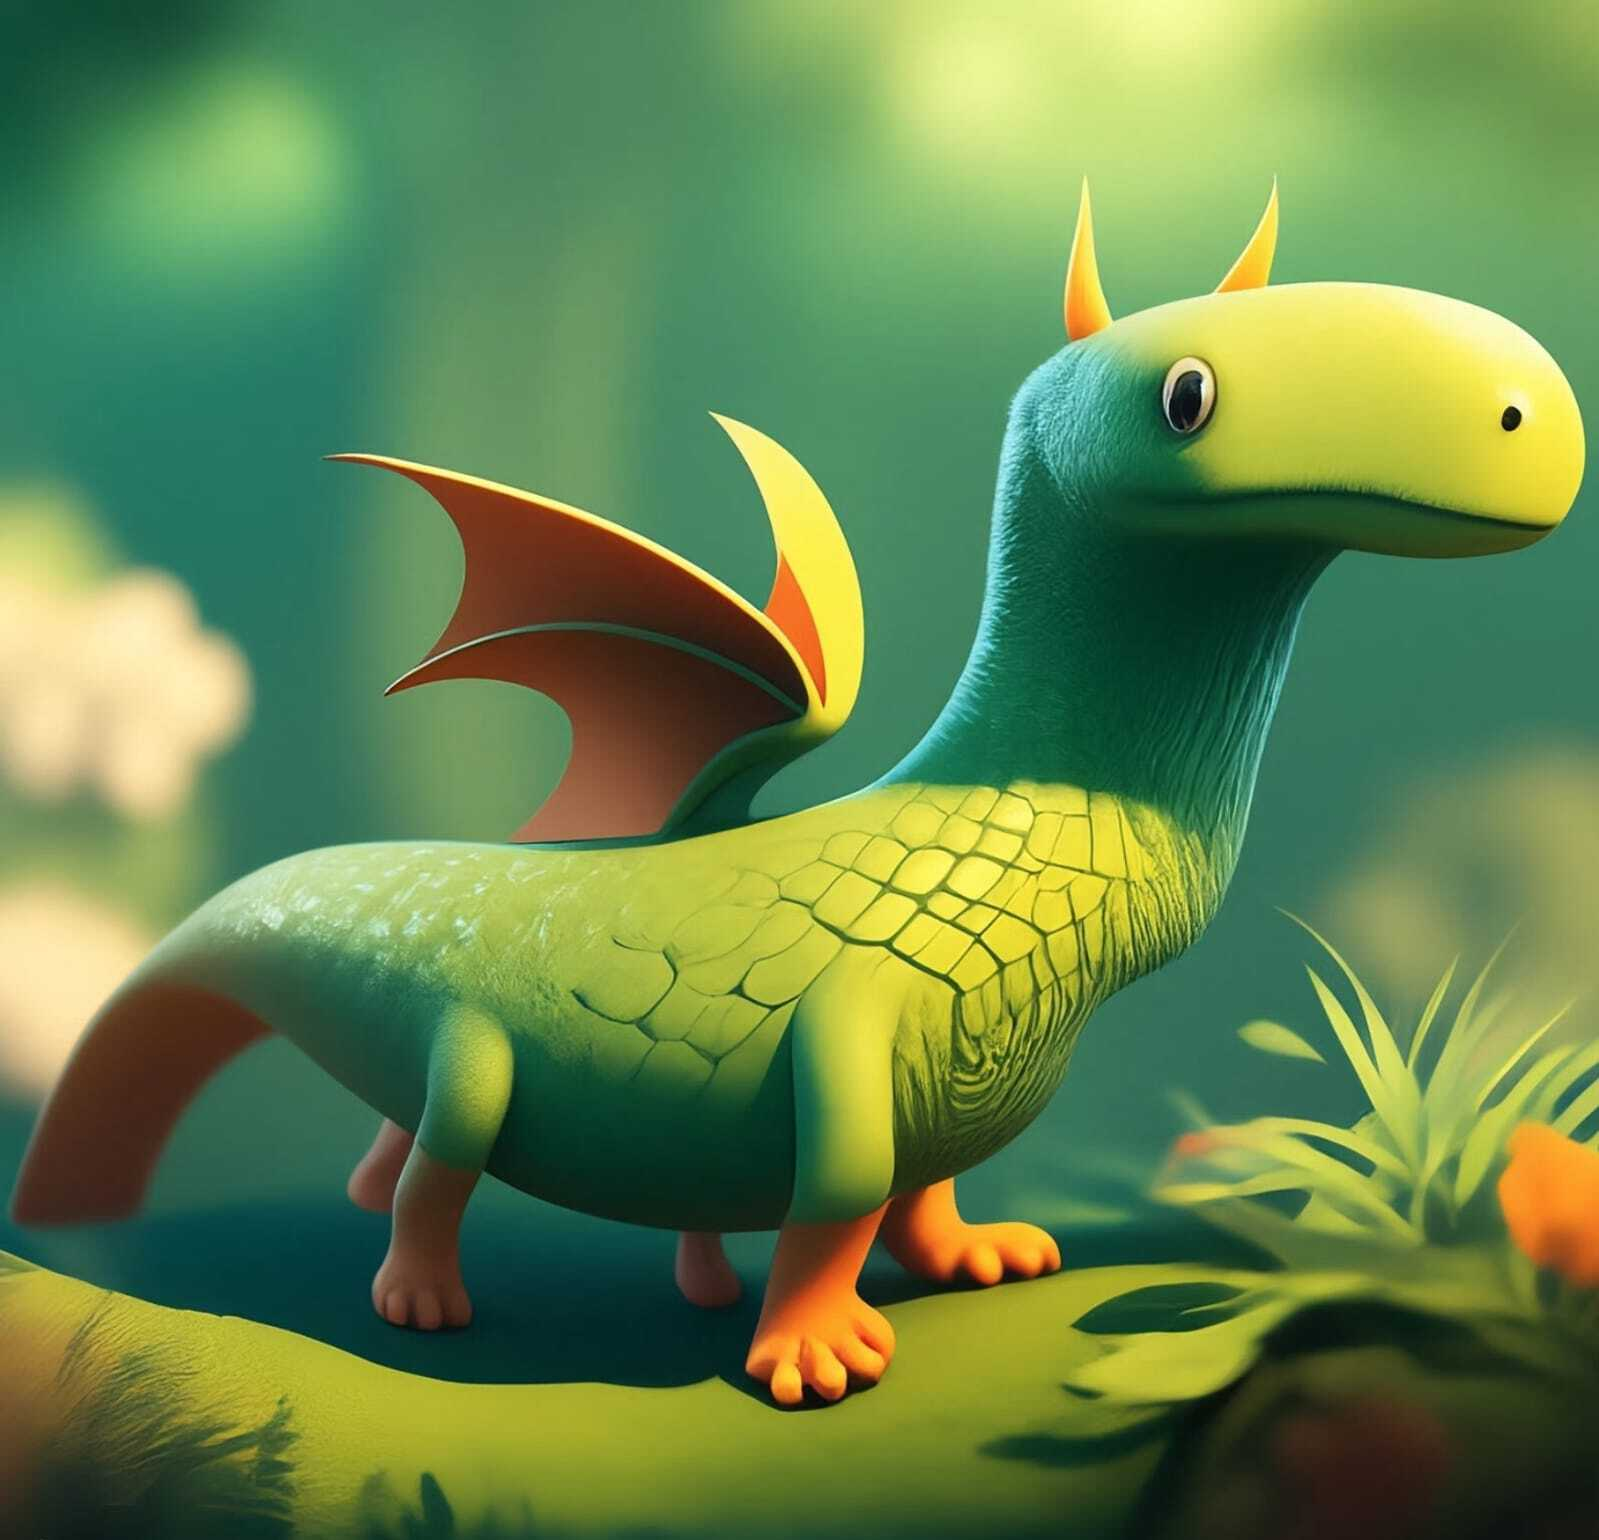
\includegraphics[width=6cm]{cover}
\end{center}
}

% theorem commands
\newtheoremstyle{c_remark}
	{}	% Space above
	{}	% Space below
	{}% Body font
	{}	% Indent amount
	{\bfseries}	% Theorem head font
	{}	% Punctuation after theorem head
	{.5em}	% Space after theorem head
	{\thmname{#1}\thmnumber{ #2}\thmnote{ \normalfont{\text{(#3)}}}}	% head content
\newtheoremstyle{c_definition}
	{3pt}	% Space above
	{3pt}	% Space below
	{}% Body font
	{}	% Indent amount
	{\bfseries}	% Theorem head font
	{}	% Punctuation after theorem head
	{.5em}	% Space after theorem head
	{\thmname{#1}\thmnumber{ #2}\thmnote{ \normalfont{\text{(#3)}}}}	% head content
\newtheoremstyle{c_plain}
	{3pt}	% Space above
	{3pt}	% Space below
	{\itshape}% Body font
	{}	% Indent amount
	{\bfseries}	% Theorem head font
	{}	% Punctuation after theorem head
	{.5em}	% Space after theorem head
	{\thmname{#1}\thmnumber{ #2}\thmnote{ \text{(#3)}}}	% head content

\ifcsname c@english\endcsname
	\theoremstyle{plain}
	\newtheorem{theorem}{Theorem}[section]
	\newtheorem{lemma}[theorem]{Lemma}
	\newtheorem{proposition}[theorem]{Proposition}
	\newtheorem*{proposition*}{Proposition}
	%\newtheorem{corollary}[theorem]{אין חלופה עברית}

	\theoremstyle{definition}
	\newtheorem{definition}[theorem]{Definition}
	\newtheorem*{definition*}{Definition}
	\newtheorem{example}{Example}[section]
	\newtheorem{exercise}{Exercise}[section]

	\theoremstyle{remark}
	\newtheorem*{remark}{Remark}
	\newtheorem*{solution}{Solution}
	\newtheorem{conclusion}[theorem]{Conclusion}
	\newtheorem{notation}[theorem]{Notation}
\else
	\theoremstyle{c_plain}
	\newtheorem{theorem}{משפט}[section]
	\newtheorem{lemma}[theorem]{למה}
	\newtheorem{proposition}[theorem]{טענה}
	\newtheorem*{proposition*}{טענה}
	%\newtheorem{corollary}[theorem]{אין חלופה עברית}

	\theoremstyle{c_definition}
	\newtheorem{definition}[theorem]{הגדרה}
	\newtheorem*{definition*}{הגדרה}
	\newtheorem{example}{דוגמה}[section]
	\newtheorem{exercise}{תרגיל}[section]

	\theoremstyle{c_remark}
	\newtheorem*{remark}{הערה}
	\newtheorem*{solution}{פתרון}
	\newtheorem{conclusion}[theorem]{מסקנה}
	\newtheorem{notation}[theorem]{סימון}
\fi

% Questions related commands
\newcounter{question}
\setcounter{question}{1}
\newcounter{sub_question}
\setcounter{sub_question}{1}

\ifcsname c@english\endcsname
	\newcommand{\question}[1][0]{
		\ifthenelse{#1 = 0}{}{\setcounter{question}{#1}}
		\section{Question \arabic{question}}
		\addtocounter{question}{1}
		\setcounter{sub_question}{1}
	}

	\newcommand{\subquestion}[1][0]{
		\ifthenelse{#1 = 0}{}{\setcounter{sub_question}{#1}}
		\subsection{Part \alph{sub_question}}
		\addtocounter{sub_question}{1}
	}
\else
	\newcommand{\question}[1][0]{
		\ifthenelse{#1 = 0}{}{\setcounter{question}{#1}}
		\section{שאלה \arabic{question}}
		\addtocounter{question}{1}
		\setcounter{sub_question}{1}
	}

	\newcommand{\subquestion}[1][0]{
		\ifthenelse{#1 = 0}{}{\setcounter{sub_question}{#1}}
		\subsection{סעיף \localecounter{letters.gershayim}{sub_question}}
		\addtocounter{sub_question}{1}
	}
\fi

% import lua and start of document
\directlua{common = require ('../common')}

\GetEnv{AUTHOR}

% headers
\author{\AUTHOR}
\date\today

\title{פתרון מטלה 07 --- תורת הקבוצות (80200)}

\DeclareMathOperator\Pfin{\mathcal{P}_\text{fin}}
\DeclareMathOperator\lex{\le_\text{lex}}
\begin{document}
\maketitle
\maketitleprint{}

\Question{}
נוכיח שאם $\langle A, \le_A \rangle$ קבוצה סדורה חלקית, אז יש שיכון של $\langle A, \le_A \rangle$ לתוך $\langle \mathcal{P}(A), \subseteq \rangle$.
\begin{proof}
	יהי איבר $b \in A$, ונגדיר $B = \{ \langle n, m \rangle \in \le_A \mid m = b \}$, ולכן $\forall c \in B : c \le b$, נגדיר $f : \langle A, \le_A \rangle \to \langle \mathcal{P}(A), \subseteq \rangle$, על־ידי
	\[
		f(x) = \{ \langle a, x \rangle \in \le_A \}
	\]
	למעשה פונקציה זו מחזירה קבוצת האיברים הקטנים מהאיבר המקורי (כולל אותו עצמו), ולכן מהתכונות של סדר נוכל להסיק $a \le_A b \implies f(a) \subseteq f(b)$ ומצאנו שיכון.
\end{proof}

\Question{}
לכל קבוצה $A$ נסמן $\Pfin(A) = \{ X \subseteq A \mid X \text{ is finite} \}$.

\Subquestion{}
נמצא שיכון של $\langle \ZZ, \le \rangle$ לתוך $\langle \mathcal{P}(\NN), \subseteq \rangle$.

נגדיר $f : \ZZ \to \NN$ על־ידי
\[
	f(z) = \begin{cases}
		2z + 1 & z \le 0 \\
		-2z & z < 0
	\end{cases}
\]
יחד עם יחס הסדר $\preceq = \{ \langle n, m \rangle \in \NN^2 \mid m = 1 (\mod 2) \implies n \le m \lor n = 0 (\mod 2) \implies n \le m \lor (n = 0 (\mod 2) \land m = 1 (\mod 2)) \}$. \\*
מהותית סדר שבודק את הזוגיות ומשמר את הסדר המקורי של $\ZZ$, ועתה נרכיב את השיכון משאלה 1 ונקבל שיכון כפי שנתבקשנו.

\Subquestion{}
נוכיח כי לא קיים שיכון של $\langle \ZZ, \le \rangle$ לתוך $\langle \Pfin(\NN), \subseteq \rangle$.
\begin{proof}
	נניח בשלילה כי ישנו שיכון $f$ כזה. \\*
	לכן $f(-1) \subseteq f(0)$, וכמו־כן גם $\forall n \in -\NN : f(n) \subseteq f(0)$, ולכן נוכל להסיק כי $|f(0)| = \aleph_0$ בסתירה להנחה כי כל איבר ב־$\Pfin(\NN)$ הוא סופי.
\end{proof}

\Subquestion{}
נמצא שיכון של $\langle Seq(\NN), \trianglelefteq \rangle$ לתוך $\langle \NN \setminus \{ 0 \}, \mid \rangle$.

נגדיר $\varphi : \NN \to \NN$ פונקציה המחזירה ראשוניים הולכים וגדלים. \\*
נגדיר $f : \langle Seq(\NN), \trianglelefteq \rangle \to \langle \NN \setminus \{ 0 \}, \mid \rangle$ על־ידי
\[
	f(\langle n_1, \dots, n_d \rangle) = \prod_{i = 1}^d \varphi({\varphi(i)}^{n_i})
\]
נניח כי $v, u \in Seq(\NN)$ כך ש־$v \trianglelefteq u$ אז נובע כי $v = \langle v_1, \dots, v_d \rangle, u = \langle v_1, \dots, v_d, u_{d + 1}, \dots, u_k \rangle$, \\*
אז נובע כי $f(u) = f(v) \cdot C$ ולכן $f(v) \mid f(u)$. \\*
בכיוון ההפוך נניח כי $f(v) \mid f(u)$ ונקבל מפירוק $f(u)$ למספרים ראשוניים וחישוב כי $v_1 = u_1$ וכן הלאה, ונוכל להסיק $v \trianglelefteq u$.

\Subquestion{}
נוכיח כי $\langle Seq(\NN), \trianglelefteq \rangle$ ו־$\langle \NN \setminus \{ 0 \}, \mid \rangle$ לא איזומורפיים.
\begin{proof}
	יהיו $a, b \in \NN$, נבחין כי קיים $c \in \NN$ כך ש־$a, b \mid c$ תמיד ($c = ab$ לדוגמה). \\*
	לעומת זאת יהיו $u, v \in Seq(\NN)$, אם $u \ne v$ והם מאותו האורך, אז אין $w \in Seq(\NN)$ כך ש־$a \trianglelefteq c$ וגם $b \trianglelefteq c$, בסתירה לשימור מקסימלי לתת־קבוצות בין קבוצות איזומורפיות.
\end{proof}

\Subquestion{}
נמצא שיכון של $\langle Seq(\NN), \trianglelefteq \rangle$ לתוך $\langle \Pfin(\NN), \subseteq\rangle$.

נשתמש בפונקציה שהגדרנו בשאלה 1, עלינו לבדוק רק שכל קבוצה שתתקבל היא אכן סופית. \\*
יהי $u \in Seq(\NN)$, ונניח כי גודל $u$ הוא $n$, אז נסיק כי $u$ גדול מ־$n$ איברים, הם הצמצומים שלו, וסדרה ריקה, ולכן $|f(u)| = n$, ולכן $f(u) \in \Pfin(\NN)$ לכל $u \in Seq(\NN)$.

\Subquestion{}
נוכיח כי $\langle Seq(\NN), \trianglelefteq \rangle$ ו־$\langle \Pfin(\NN), \subseteq\rangle$ לא איזומורפיים.
\begin{proof}
	למעשה, ההוכחה זהה לסעיף ד', שכן לכל שתי קבוצות $X, Y \in \Pfin(\NN)$ קיים $X \cup Y$ אשר מהווה איבר גדול משתיהן. \\*
	לעומת זאת, ראינו כי לא לכל שני איברים יש איבר משותף גדול משניהם ב־$Seq(\NN)$.
\end{proof}

\Question{}
הגדרנו עבור סדרים חלקיים $\langle A, \le_A \rangle, \langle B, \le_B \rangle$ את הסדר המילוני על $A \times B$ על־ידי
\[
	\langle a, b \rangle \lex \langle a', b' \rangle \iff a <_A a' \lor (a = a' \land b \le_B b')
\]
נניח כי $A, B$ קבוצות לא ריקות.

\Subquestion{}
נוכיח כי $\langle A \times B, \lex \rangle$ קבוצה סדורה חלקית.
\begin{proof}
	נבדוק את תכונות הסדר החלקי:
	\begin{enumerate}
		\item רפלקסיביות: $\forall (a, b) \in A \times B \implies a = a' \land b \le_B b \iff \langle a, b \rangle \lex \langle a, b \rangle$.
		\item טרנזיטיבי: $\forall \langle a_1, b_1 \rangle, \langle a_2, b_2 \rangle, \langle a_3, b_3 \rangle \in A \times B : \langle a_1, b_1 \rangle \lex \langle a_2, b_2 \rangle \land \langle a_2, b_2 \lex \langle a_3, b_3 \rangle \iff (a_1 <_A a_2 \lor (a_1 = a_2 \land b_1 \le_B b_2)) \land (a_2 <_A a_3 \lor (a_2 = a_3 \land b_2 \le_B b_3)) \iff (a_1 <_A a2 \land a_2 <_A a_3) \lor (a_1 = a_2 \land b_2 \le_B b_3 \land a_2 = a_3 \land b_2 \le_B b_3) \iff (a_1 <_A a_3) \lor (a_1 = a_3 \land b_1 \le_B b_3) \iff \langle a_1, b_1 \rangle \lex \langle a_3, b_3 \rangle$.
		\item אנטי־סימטרי: $\forall \langle a, b \rangle, \langle a', b' \rangle \in A \times B : \langle a, b \rangle \lex \langle a', b' \rangle \land \langle a', b' \rangle \lex \langle a, b \rangle \iff (a < a' \land a' < a) \lor (a = a' \land (b \le b' \land b' \le b)) \iff a = a' \land b = b' \iff \langle a, b \rangle = \langle a', b' \rangle$.
	\end{enumerate}
	ומצאנו כי שלושת התנאים מתקיימים וזהו אכן יחס סדר חלקי.
\end{proof}

\Subquestion{}
נוכיח כי $\langle A \times B, \lex \rangle$ סדורה קווית אם ורק אם $\langle A, \le_A \rangle, \langle B, \le_B \rangle$ סדורות קווית.
\begin{proof}
	\textbf{כיוון ראשון:}
	נניח כי $\langle A \times B, \lex \rangle$ סדורה קווית. \\*
	נבחן את $\langle a, b \rangle, \langle a', b \rangle$, אם הם שווים נובע $a = a'$,
	אם $\langle a, b \rangle \lex \langle a', b \rangle$ אז נובע $a \le_A a$ ואם $\langle a', b \rangle \lex \langle a, b \rangle$ אז באופן דומה נקבל $a' \le_A a$.
	קיבלנו כי $\langle A, \le_A \rangle$ קווית, ובאותו אופן בדיוק עבור $\langle a, b \rangle, \langle a, b' \rangle$ נקבל כי גם $\langle B, \le_B \rangle$ קווית.

	\textbf{כיוון שני:}
	נניח כי $\langle A, \le_A \rangle, \langle B, \le_B \rangle$ שניהם סדרים קוויים. \\*
	נבחן את $\langle a, b \rangle, \langle a', b' \rangle$, אם $a = a', b = b'$ אז גם $\langle a, b \rangle = \langle a', b' \rangle$. \\*
	אם $a \le_A a' \land b \le_B b'$ אז נובע כי $a <_A a'$ או $a = a'$ ולכן $\langle a, b \rangle \lex \langle a', b' \rangle$. \\*
	אם $a' \le_A a \land b' \le_B b$ אז באופן זהה השוויון מתקיים לכיוון השני. \\*
	אם $a <_A a'$ אז כמובן היחס מתקיים, וגם $a >_A a'$, ולכן נניח ש־$a = a'$. \\*
	אם $b \le_B b'$ אז $\langle a, b \rangle \lex \langle a', b' \rangle$, הכיוון השני זהה, וסיימנו לעבור על כל המקרים וראינו כי תמיד היחס מוגדר, ובהתאם היחס קווי.
\end{proof}

\Subquestion{}
נוכיח כי $\langle A \times B, \lex \rangle$ מבוסס היטב אם ורק אם $\langle A, \le_A \rangle, \langle B, \le_B \rangle$ מבוססים היטב שניהם.
\begin{proof}
	\textbf{כיוון ראשון:}
	נניח כי $\langle A \times B, \lex \rangle$ מבוסס היטב. \\*
	לכל תת־קבוצה $A' \subseteq A$ נקבל כי לקבוצה $A' \times \{ b \}$ (כאשר $b$ קבוע) יש איבר מינימלי. תחת ההגבלה נקבל כי $\lex \iff a <_A a' \lor a = a' \iff a \le_A a' \iff \le_A$,
	דהינו נקבל כי לכל $A' \subseteq A$ לא ריקה קיים איבר מינימלי עבור $\le_A$ ולכן $\langle A, \le_A \rangle$ מבוסס היטב. \\*
	ההוכחה ל־$B$ זהה לחלוטין ונובעת מהעובדה ש־$\langle a, b \rangle \lex \langle a, b' \rangle \iff b \le_B b'$.

	\textbf{כיוון שני:}
	נניח כי $\langle A, \le_A \rangle, \langle \langle B, \le_B \rangle$ סדרים מבוססים היטב, ותהינה $A' \subseteq A, B' \subseteq B$ כאשר $A', b' \ne \emptyset$. \\*
	לכן קיימים איברים מינימליים $a \in A', b \in B'$.
	נבדוק עתה את $\langle a', b' \rangle \in A' \times B'$ איבר כלשהו. \\*
	נניח ש־$\langle a', b' \rangle \lex \langle a, b \rangle$ ולכן נקבל $a \le_A a' \land b \le_B b' \land (a' <_A a \lor (a' = a \land b' \le_B b)) \iff a = a' \land b = b'$ ולכן $\langle a, b \rangle$ מינימלי ב־$A' \times B'$.
\end{proof}

\Question{}
נוכיח כי לכל $n, m \in \NN$ מתקיים $\langle [n] \times [m], \lex \rangle \cong \langle [n \cdot m ], \le \rangle$.
\begin{proof}
	נתחיל במציאת שיכון בין הסדרים. \\*
	נגדיר $f : \langle [n] \times [m], \lex \rangle \to \langle [n \cdot m ], \le \rangle$ על־ידי
	\[
		f(x, y) = mx + y
	\]
	ונקבל $\forall \langle x, y \rangle, \langle x', y' \rangle \in [n] \times [m] : \langle x, y \rangle \lex \langle x', y' \rangle \iff x < x' \lor (x = x' \land y \le y') \iff mx < mx' \lor (nx + y \le mx' + y') \iff mx + y \le mx' + y' \iff f(x, y) \lex f(x', y')$ כנביעה מ־$y < m$. \\*
	נבחין עתה כי כל $z \in [n \cdot m ]$ ניתן לייצוג על־ידי $z = mx + y$ ולכן נוכל לקבוע כי $f$ היא על ובהתאם $\langle [n] \times [m], \lex \rangle \cong \langle [n \cdot m ], \le \rangle$.
\end{proof}

\directlua{Q_number = 6}
\Question{}
נניח כי $\langle A, \le \rangle$ סדר קווי צפוף ללא מקסימום ומינימום. \\*
יהיו $\langle B, \le_B \rangle, \langle B', \le_{B'} \rangle$ סדרים קוויים שלמים ללא מינימום ומקסימום. \\*
$g : A \to B, g' : A \to B'$ שיכונים של הסדרים כך ש־$\rng(g), \rng(g')$ צפופים ב־$B, B'$ בהתאמה. \\*
נוכיח שקיים איזומורפיזם יחיד של סדרים $h : B \to B'$ המקיים $h \circ g = g'$.
\begin{proof}
	אנחנו יודעים כי $B, B'$ שתיהן סדרים שלמים וצפופים, ולכן לשתיהן יש סופרמום ואינפימום.
	מצטער, אני לא יודע לעשות את השאלה הזאת בלי בחירה.
	נבחר $x_0 \in B, y_0 \in B'$ ונגדיר פונקציה $h : B \to B'$ כך ש־$f(x_0) = y_0$. \\*
	לצורך ההוכחה ''נוסיף'' שני איברים המייצגים מינימום ומקסימום לשתי הקבוצות, $s, s', i, i'$ מקסימום ואינפימום בהתאמה, ונגדיר $h(s) = s', h(i) = i'$. \\*
	עתה לכל $i < x < x_0 < x' < s$ נבחר $i' < y < y_0 < y' < s'$ כלשהם ונגדיר $h(x) = y, h(x') = y'$, ננצל את אקסיומת הבחירה ונבנה את הפונקציה ככה לכל $x \in B$. \\*
	קיבלנו שיכון, שכן $x \le_B x' \iff h(x) \le_{B'} h(x')$ ישירות מהגדרת הפונקציה. \\*
	נוכל עתה להסיר את האיברים מהקבוצות ולשמר את מבנה הפונקציה מעבר לשני איברים אלה וקיבלנו שיכון בין $B$ ו־$B'$ כקבוצות שקיבלנו. \\*
	נבחין כי $h$ חד־חד ערכית, אבל גם על על־פי הגדרתנו, שכן לכל איבר $y \in B'$ בחרנו איבר $x \in B$ אשר מקיים את השיכון בצפיפות.

	מצאנו כי קיימים איזומורפיזמים בין $B, B'$, ומצאנו כי נוכל לבנות אותם על־פי קבוצות איברים ב־$B, B'$, ולכן עתה נבחן את $A$ ואת $g, g'$. \\*
	אנו יודעים כי $\rng(B), \rng(B')$ הן צפופות ונוכל להסיק שאין להן מינימום ומקסימום, שכן אחרת נקבל סתירה להגדרת $A$, ולכן נבנה את $h$ כך ש־$\rng(B) \cong \rng(B')$. \\*
	קיבלנו אם כן כי $h \circ g = g'$, ונשאר לנו להוכיח כי $h$ יחידה. \\*
	למעשה שוויון זה מאלץ כבר יחידות, שכן מדובר באיזומורפיזמים, אין איברים חופשיים ל־$h$ שלא מעבירים איבר מ־$B$ ל־$B'$ (לצמצומם).
\end{proof}

\end{document}
